\par O valor do nó corresponde à $h(s)+c(s)$, onde $h(s)$ é o valor da heurística do nó e $c(s)$ é o custo.

\par \hfil 
\resizebox{\linewidth}{!}{\begin{tikzpicture}

  \node[label=left:{\small 4}] (a) {
    \begin{tikzpicture}
      \draw [rounded corners=1pt] (0,0) rectangle ++(2.5,0.5);
      \draw[fill=black] (0.25,0.25) circle (5pt);
      \draw[fill=black] (0.75,0.25) circle (5pt);
      \draw (1.25,0.25) circle (5pt);
      \draw (1.75,0.25) circle (5pt);
    \end{tikzpicture}
  };

  %-------------
  % NÍVEL 1
  %-------------
  \node[label=left:{\small 5}, below left=of a] (b) {
    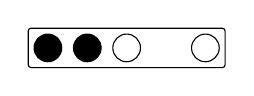
\begin{tikzpicture}
      \draw [rounded corners=1pt] (0,0) rectangle ++(2.5,0.5);
      \draw[fill=black] (0.25,0.25) circle (5pt);
      \draw[fill=black] (0.75,0.25) circle (5pt);
      \draw (1.25,0.25) circle (5pt);
      \draw (2.25,0.25) circle (5pt);
    \end{tikzpicture}
  };

  \node[label=right:{\small 6}, below right=of a] (c) {
    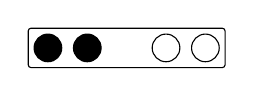
\begin{tikzpicture}
      \draw [rounded corners=1pt] (0,0) rectangle ++(2.5,0.5);
      \draw[fill=black] (0.25,0.25) circle (5pt);
      \draw[fill=black] (0.75,0.25) circle (5pt);
      \draw (1.75,0.25) circle (5pt);
      \draw (2.25,0.25) circle (5pt);
    \end{tikzpicture}
  };

  %------------
  % NÍVEL 2
  %------------

  \node[label=left:{\small 6}, below=of b] (d) {
    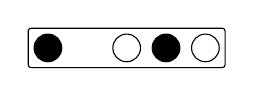
\begin{tikzpicture}
      \draw [rounded corners=1pt] (0,0) rectangle ++(2.5,0.5);
      \draw[fill=black] (0.25,0.25) circle (5pt);
      \draw[fill=black] (1.75,0.25) circle (5pt);
      \draw (1.25,0.25) circle (5pt);
      \draw (2.25,0.25) circle (5pt);
    \end{tikzpicture}
  };

  \node[label=left:{\small 8}, below=of c] (g) {
    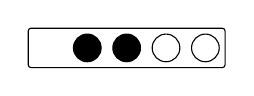
\begin{tikzpicture}
      \draw [rounded corners=1pt] (0,0) rectangle ++(2.5,0.5);
      \draw[fill=black] (1.25,0.25) circle (5pt);
      \draw[fill=black] (0.75,0.25) circle (5pt);
      \draw (1.75,0.25) circle (5pt);
      \draw (2.25,0.25) circle (5pt);
    \end{tikzpicture}
  };

  \node[label=right:{\small 7}, below right=of c] (h) {
    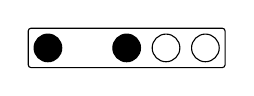
\begin{tikzpicture}
      \draw [rounded corners=1pt] (0,0) rectangle ++(2.5,0.5);
      \draw[fill=black] (0.25,0.25) circle (5pt);
      \draw[fill=black] (1.25,0.25) circle (5pt);
      \draw (1.75,0.25) circle (5pt);
      \draw (2.25,0.25) circle (5pt);
    \end{tikzpicture}
  };

  %------------
  % NÍVEL 3
  %------------

  \node[label=left:{\small 7}, below left=of d] (e) {
    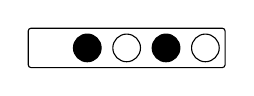
\begin{tikzpicture}
      \draw [rounded corners=1pt] (0,0) rectangle ++(2.5,0.5);
      \draw[fill=black] (0.75,0.25) circle (5pt);
      \draw[fill=black] (1.75,0.25) circle (5pt);
      \draw (1.25,0.25) circle (5pt);
      \draw (2.25,0.25) circle (5pt);
    \end{tikzpicture}
  };

  \node[label=right:{\small 7}, below=of d] (f) {
    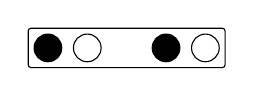
\begin{tikzpicture}
      \draw [rounded corners=1pt] (0,0) rectangle ++(2.5,0.5);
      \draw[fill=black] (0.25,0.25) circle (5pt);
      \draw[fill=black] (1.75,0.25) circle (5pt);
      \draw (0.75,0.25) circle (5pt);
      \draw (2.25,0.25) circle (5pt);
    \end{tikzpicture}
  };

  %------------
  % NÍVEL 4
  %------------

  \node[label=left:{\small 8}, below=of e] (i) {
    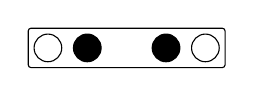
\begin{tikzpicture}
      \draw [rounded corners=1pt] (0,0) rectangle ++(2.5,0.5);
      \draw[fill=black] (0.75,0.25) circle (5pt);
      \draw[fill=black] (1.75,0.25) circle (5pt);
      \draw (0.25,0.25) circle (5pt);
      \draw (2.25,0.25) circle (5pt);
    \end{tikzpicture}
  };

  \node[label=right:{\small 8}, below=of f] (j) {
    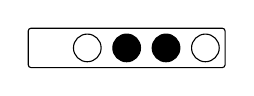
\begin{tikzpicture}
      \draw [rounded corners=1pt] (0,0) rectangle ++(2.5,0.5);
      \draw[fill=black] (1.25,0.25) circle (5pt);
      \draw[fill=black] (1.75,0.25) circle (5pt);
      \draw (0.75,0.25) circle (5pt);
      \draw (2.25,0.25) circle (5pt);
    \end{tikzpicture}
  };

  \node[label=right:{\small 8}, below right=of f] (k) {
    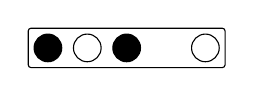
\begin{tikzpicture}
      \draw [rounded corners=1pt] (0,0) rectangle ++(2.5,0.5);
      \draw[fill=black] (0.25,0.25) circle (5pt);
      \draw[fill=black] (1.25,0.25) circle (5pt);
      \draw (0.75,0.25) circle (5pt);
      \draw (2.25,0.25) circle (5pt);
    \end{tikzpicture}
  };

  \node[label=right:{\small 8}, right=of k] (l) {
    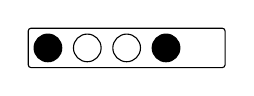
\begin{tikzpicture}
      \draw [rounded corners=1pt] (0,0) rectangle ++(2.5,0.5);
      \draw[fill=black] (0.25,0.25) circle (5pt);
      \draw[fill=black] (1.75,0.25) circle (5pt);
      \draw (0.75,0.25) circle (5pt);
      \draw (1.25,0.25) circle (5pt);
    \end{tikzpicture}
  };

  %------------
  % NÍVEL 5
  %------------

  \node[label=left:{\small 9}, below left=of i] (m) {
    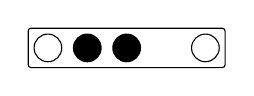
\begin{tikzpicture}
      \draw [rounded corners=1pt] (0,0) rectangle ++(2.5,0.5);
      \draw[fill=black] (0.75,0.25) circle (5pt);
      \draw[fill=black] (1.25,0.25) circle (5pt);
      \draw (0.25,0.25) circle (5pt);
      \draw (2.25,0.25) circle (5pt);
    \end{tikzpicture}
  };

  \node[label=left:{\small 9}, left=of m] (n) {
    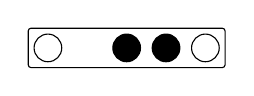
\begin{tikzpicture}
      \draw [rounded corners=1pt] (0,0) rectangle ++(2.5,0.5);
      \draw[fill=black] (1.75,0.25) circle (5pt);
      \draw[fill=black] (1.25,0.25) circle (5pt);
      \draw (0.25,0.25) circle (5pt);
      \draw (2.25,0.25) circle (5pt);
    \end{tikzpicture}
  };

  \node[label=right:{\small 11}, below=of i] (o) {
    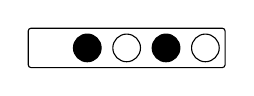
\begin{tikzpicture}
      \draw [rounded corners=1pt] (0,0) rectangle ++(2.5,0.5);
      \draw[fill=black] (0.75,0.25) circle (5pt);
      \draw[fill=black] (1.75,0.25) circle (5pt);
      \draw (1.25,0.25) circle (5pt);
      \draw (2.25,0.25) circle (5pt);
    \end{tikzpicture}
  };

  \node[label=right:{\small 9}, below left=of k] (p) {
    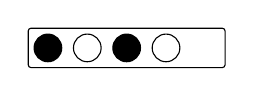
\begin{tikzpicture}
      \draw [rounded corners=1pt] (0,0) rectangle ++(2.5,0.5);
      \draw[fill=black] (0.25,0.25) circle (5pt);
      \draw[fill=black] (1.25,0.25) circle (5pt);
      \draw (0.75,0.25) circle (5pt);
      \draw (1.75,0.25) circle (5pt);
    \end{tikzpicture}
  };

  \node[label=right:{\small 11}, below=of k] (q) {
    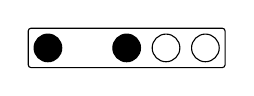
\begin{tikzpicture}
      \draw [rounded corners=1pt] (0,0) rectangle ++(2.5,0.5);
      \draw[fill=black] (0.25,0.25) circle (5pt);
      \draw[fill=black] (1.25,0.25) circle (5pt);
      \draw (2.25,0.25) circle (5pt);
      \draw (1.75,0.25) circle (5pt);
    \end{tikzpicture}
  };

  \node[label=right:{\small 10}, below=of l] (r) {
    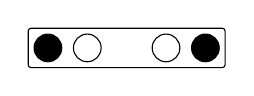
\begin{tikzpicture}
      \draw [rounded corners=1pt] (0,0) rectangle ++(2.5,0.5);
      \draw[fill=black] (0.25,0.25) circle (5pt);
      \draw[fill=black] (2.25,0.25) circle (5pt);
      \draw (0.75,0.25) circle (5pt);
      \draw (1.75,0.25) circle (5pt);
    \end{tikzpicture}
  };

  %------------
  % NÍVEL 6
  %------------

  \node[label=right:{\small 11}, below=of r] (s) {
    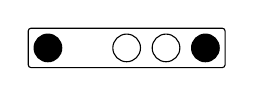
\begin{tikzpicture}
      \draw [rounded corners=1pt] (0,0) rectangle ++(2.5,0.5);
      \draw[fill=black] (0.25,0.25) circle (5pt);
      \draw[fill=black] (2.25,0.25) circle (5pt);
      \draw (1.25,0.25) circle (5pt);
      \draw (1.75,0.25) circle (5pt);
    \end{tikzpicture}
  };

  \node[label=right:{\small 11}, below left=of r] (t) {
    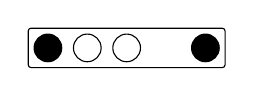
\begin{tikzpicture}
      \draw [rounded corners=1pt] (0,0) rectangle ++(2.5,0.5);
      \draw[fill=black] (0.25,0.25) circle (5pt);
      \draw[fill=black] (2.25,0.25) circle (5pt);
      \draw (1.25,0.25) circle (5pt);
      \draw (0.75,0.25) circle (5pt);
    \end{tikzpicture}
  };


  %------------
  % NÍVEL 7
  %------------

  \node[label=right:{\small 12}, below=of s] (u) {
    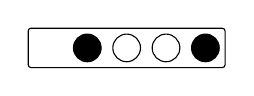
\begin{tikzpicture}
      \draw [rounded corners=1pt] (0,0) rectangle ++(2.5,0.5);
      \draw[fill=black] (0.75,0.25) circle (5pt);
      \draw[fill=black] (2.25,0.25) circle (5pt);
      \draw (1.75,0.25) circle (5pt);
      \draw (1.25,0.25) circle (5pt);
    \end{tikzpicture}
     };

  %------------
  % NÍVEL 8
  %------------

  \node[label=right:{\small 13}, below=of u] (v) {
    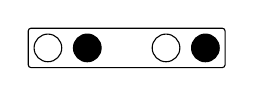
\begin{tikzpicture}
      \draw [rounded corners=1pt] (0,0) rectangle ++(2.5,0.5);
      \draw[fill=black] (0.75,0.25) circle (5pt);
      \draw[fill=black] (2.25,0.25) circle (5pt);
      \draw (1.75,0.25) circle (5pt);
      \draw (0.25,0.25) circle (5pt);
    \end{tikzpicture}
  };

  %------------
  % NÍVEL 8
  %------------

  \node[label=right:{\small 14}, below left=of v] (w) {
    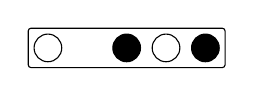
\begin{tikzpicture}
      \draw [rounded corners=1pt] (0,0) rectangle ++(2.5,0.5);
      \draw[fill=black] (1.25,0.25) circle (5pt);
      \draw[fill=black] (2.25,0.25) circle (5pt);
      \draw (1.75,0.25) circle (5pt);
      \draw (0.25,0.25) circle (5pt);
    \end{tikzpicture}
  };

  \node[label=right:{\small 14}, below=of v] (x) {
    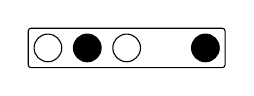
\begin{tikzpicture}
      \draw [rounded corners=1pt] (0,0) rectangle ++(2.5,0.5);
      \draw[fill=black] (0.75,0.25) circle (5pt);
      \draw[fill=black] (2.25,0.25) circle (5pt);
      \draw (1.25,0.25) circle (5pt);
      \draw (0.25,0.25) circle (5pt);
    \end{tikzpicture}
  };

  %------------
  % NÍVEL 9
  %------------

  \node[label=right:{\small 15}, below=of w] (y) {
    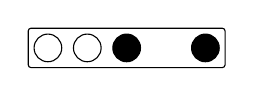
\begin{tikzpicture}
      \draw [rounded corners=1pt] (0,0) rectangle ++(2.5,0.5);
      \draw[fill=black] (1.25,0.25) circle (5pt);
      \draw[fill=black] (2.25,0.25) circle (5pt);
      \draw (0.75,0.25) circle (5pt);
      \draw (0.25,0.25) circle (5pt);
    \end{tikzpicture}
  };

  \node[label=right:{\small 15}, below=of x] (z) {
    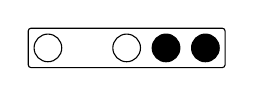
\begin{tikzpicture}
      \draw [rounded corners=1pt] (0,0) rectangle ++(2.5,0.5);
      \draw[fill=black] (1.75,0.25) circle (5pt);
      \draw[fill=black] (2.25,0.25) circle (5pt);
      \draw (1.25,0.25) circle (5pt);
      \draw (0.25,0.25) circle (5pt);
    \end{tikzpicture}
  };


  \draw (a) edge[->] node[above] {1} (b);
  \draw (a) edge[->] node[above] {2} (c);
  \draw (b) edge[->] node[left]  {2} (d);
  \draw (d) edge[->] node[above] {1} (e);
  \draw (d) edge[->] node[right] {1} (f);
  \draw (e) edge[->] node[right] {2} (i);

  \draw (f) edge[->] node[right] {2} (j);
  \draw (f) edge[->] node[below] {1} (k);
  \draw (f) edge[->] node[above] {2} (l);

  \draw (i) edge[->] node[below] {1} (m);
  \draw (i) edge[->] node[above] {1} (n);
  \draw (i) edge[->] node[right] {2} (o);

  \draw (k) edge[->] node[above] {1} (p);
  \draw (k) edge[->] node[right] {2} (q);

  \draw (l) edge[->] node[right] {2} (r);

  \draw (r) edge[->] node[right] {1} (s);
  \draw (r) edge[->] node[above] {1} (t);

  \draw (s) edge[->] node[right] {1} (u);
  \draw (u) edge[->] node[right] {2} (v);

  \draw (v) edge[->] node[above] {1} (w);
  \draw (v) edge[->] node[right] {1} (x);

  \draw (w) edge[->] node[left] {2} (y);
  \draw (x) edge[->] node[right] {2} (z);

  \draw (c) edge[->] node[left] {2} (g);
  \draw (c) edge[->] node[above] {1} (h);

\end{tikzpicture}}